% Source: nn_bigram_modeling.tex
\begin{notechapter}
\chapter{A One-Hidden-Layer Neural Bigram Model}\label{ch:bigram-neural}

\section{Introduction}
This document explains a neural network with one hidden layer of size \( D \)
applied to bigram language modeling. The goal is to estimate the probability
\( P(\text{word}_2 \mid \text{word}_1) \), where \(\text{word}_1\) is the
previous word and \(\text{word}_2\) is the next word. The model uses a hidden
layer with \( D \) neurons, a \(\tanh\) activation function, and a softmax
output layer.

\section{Model Diagram}
The following diagram illustrates the structure of the model:

\begin{center}
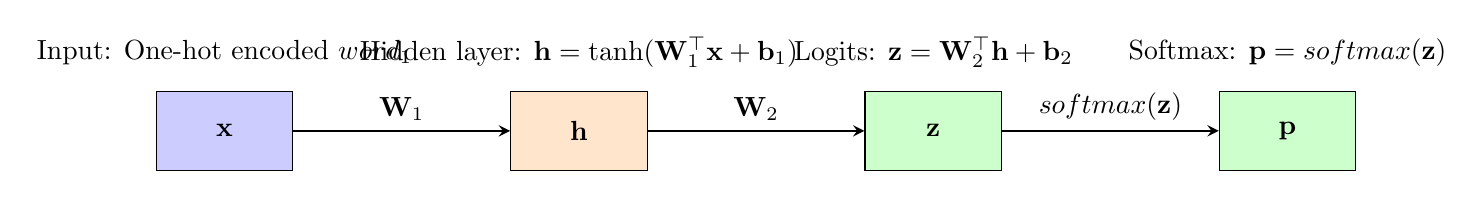
\begin{tikzpicture}[
    node distance=1.5cm,
    input/.style={rectangle, draw, fill=blue!20, text width=1.5cm, text centered, minimum height=1cm},
    hidden/.style={rectangle, draw, fill=orange!20, text width=1.5cm, text centered, minimum height=1cm},
    output/.style={rectangle, draw, fill=green!20, text width=1.5cm, text centered, minimum height=1cm},
    param/.style={rectangle, draw, fill=red!20, text width=1.5cm, text centered, minimum height=1cm},
    arrow/.style={thick,->,>=stealth}
]
    % Input layer
    \node[input] (x) {$\mathbf{x}$};
    \node[above of=x, yshift=-0.5cm] (input_label) {Input: One-hot encoded $\text{word}_1$};

    % Hidden layer
    \node[hidden, right of=x, xshift=3cm] (h) {$\mathbf{h}$};
    \node[above of=h, yshift=-0.5cm] (h_label) {Hidden layer: $\mathbf{h} = \tanh(\mathbf{W}_1^\top \mathbf{x} + \mathbf{b}_1)$};

    % Output layer
    \node[output, right of=h, xshift=3cm] (z) {$\mathbf{z}$};
    \node[above of=z, yshift=-0.5cm] (z_label) {Logits: $\mathbf{z} = \mathbf{W}_2^\top \mathbf{h} + \mathbf{b}_2$};

    % Softmax
    \node[output, right of=z, xshift=3cm] (p) {$\mathbf{p}$};
    \node[above of=p, yshift=-0.5cm] (p_label) {Softmax: $\mathbf{p} = \text{softmax}(\mathbf{z})$};

    % Arrows
    \draw[arrow] (x) -- (h) node[midway, above] {$\mathbf{W}_1$};
    \draw[arrow] (h) -- (z) node[midway, above] {$\mathbf{W}_2$};
    \draw[arrow] (z) -- (p) node[midway, above] {$\text{softmax}(\mathbf{z})$};

\end{tikzpicture}
\end{center}

\subsection{Explanation of the Diagram}
\begin{itemize}
    \item The input \(\mathbf{x}\) is a one-hot encoded vector representing
          \(\text{word}_1\).
    \item The hidden layer \(\mathbf{h}\) is computed using a weight matrix
          \(\mathbf{W}_1\) and bias \(\mathbf{b}_1\), followed by the \(\tanh\)
          activation function.
    \item The output layer \(\mathbf{z}\) is computed using a weight matrix
          \(\mathbf{W}_2\) and bias \(\mathbf{b}_2\).
    \item The softmax function converts the logits \(\mathbf{z}\) into
          probabilities \(\mathbf{p}\).
\end{itemize}

\section{Problem Setup}
The goal is to estimate the probability \( P(\text{word}_2 \mid \text{word}_1) \),
where \(\text{word}_1\) is the previous word and \(\text{word}_2\) is the next
word. The input is a one-hot encoded vector representing \(\text{word}_1\), and
the output is a probability distribution over the vocabulary for \(\text{word}_2\).

\section{Notation}
\begin{itemize}
    \item Let the vocabulary size be \( V \).
    \item Let \(\mathbf{x} \in \mathbb{R}^V\) be the one-hot encoded input
          vector for \(\text{word}_1\).
    \item Let \(\mathbf{W}_1 \in \mathbb{R}^{V \times D}\) be the weight matrix
          for the hidden layer.
    \item Let \(\mathbf{b}_1 \in \mathbb{R}^D\) be the bias for the hidden layer.
    \item Let \(\mathbf{W}_2 \in \mathbb{R}^{D \times V}\) be the weight matrix
          for the output layer.
    \item Let \(\mathbf{b}_2 \in \mathbb{R}^V\) be the bias for the output layer.
    \item Let \(\mathbf{h} \in \mathbb{R}^D\) be the hidden layer activations.
    \item Let \(\mathbf{z} \in \mathbb{R}^V\) be the logits (unnormalized scores).
\end{itemize}

\section{Forward Pass}
\begin{itemize}
    \item Compute the hidden layer activations:
          \[
          \mathbf{h} = \tanh(\mathbf{W}_1^\top \mathbf{x} + \mathbf{b}_1).
          \]
    \item Compute the logits:
          \[
          \mathbf{z} = \mathbf{W}_2^\top \mathbf{h} + \mathbf{b}_2.
          \]
    \item Apply the softmax function to convert logits \(\mathbf{z}\) into
          probabilities:
          \[
          P(\text{word}_2 = j \mid \text{word}_1) =
          \text{softmax}(\mathbf{z})_j = \frac{e^{z_j}}{\sum_{k=1}^V e^{z_k}}.
          \]
\end{itemize}

\section{Training}
The model is trained using \textbf{cross-entropy loss}. For a single training
example \((\text{word}_1, \text{word}_2)\), the loss is:
\[
\mathcal{L} = -\log P(\text{word}_2 \mid \text{word}_1).
\]
If \(\text{word}_2\) is the \(j\)-th word in the vocabulary, then:
\[
\mathcal{L} = -\log \left( \text{softmax}(\mathbf{z})_j \right).
\]
The gradients of the loss with respect to the parameters (\(\mathbf{W}_1, \mathbf{W}_2, \mathbf{b}_1, \mathbf{b}_2\)) are computed using backpropagation.

\section{Gradient Computation}
\subsection{Gradient of the Loss with Respect to the Logits}
The gradient of the cross-entropy loss with respect to the logits \(\mathbf{z}\)
is derived as follows:

\subsubsection{Softmax Function}
The softmax function is applied to the logits \(\mathbf{z}\) to compute the
probabilities:
\[
p_j = \text{softmax}(z_j) = \frac{e^{z_j}}{\sum_{k=1}^V e^{z_k}}.
\]

\subsubsection{Cross-Entropy Loss}
The cross-entropy loss for a single training example is:
\[
\mathcal{L} = -\log p_j,
\]
where \(j\) is the index of the true word \(\text{word}_2\).

\subsubsection{Derivative of the Loss}
The derivative of the loss with respect to the logits \(\mathbf{z}\) is:
\[
\frac{\partial \mathcal{L}}{\partial z_j} = p_j - \mathbb{I}(\text{word}_2 = j),
\]
where:
\begin{itemize}
    \item \(p_j\) is the predicted probability for the \(j\)-th word.
    \item \(\mathbb{I}(\text{word}_2 = j)\) is an indicator function that is 1
          if \(\text{word}_2\) is the \(j\)-th word and 0 otherwise.
\end{itemize}

This can be written in vector form as:
\[
\frac{\partial \mathcal{L}}{\partial \mathbf{z}} = \mathbf{p} - \mathbf{y},
\]
where \(\mathbf{y}\) is the one-hot encoded vector for \(\text{word}_2\).

\subsection{Gradient with Respect to the Output Layer Parameters}
The gradients of the loss with respect to \(\mathbf{W}_2\) and \(\mathbf{b}_2\)
are computed as follows:

\subsubsection{Logits Computation}
The logits \(\mathbf{z}\) are computed as:
\[
\mathbf{z} = \mathbf{W}_2^\top \mathbf{h} + \mathbf{b}_2.
\]

\subsubsection{Gradient with Respect to \(\mathbf{W}_2\)}
The gradient of the loss with respect to \(\mathbf{W}_2\) is:
\[
\frac{\partial \mathcal{L}}{\partial \mathbf{W}_2} =
\frac{\partial \mathcal{L}}{\partial \mathbf{z}} \cdot \mathbf{h}^\top.
\]
This is because \(\mathbf{z}\) depends on \(\mathbf{W}_2\) through the matrix
multiplication \(\mathbf{W}_2^\top \mathbf{h}\).

\subsubsection{Gradient with Respect to \(\mathbf{b}_2\)}
The gradient of the loss with respect to \(\mathbf{b}_2\) is:
\[
\frac{\partial \mathcal{L}}{\partial \mathbf{b}_2} =
\frac{\partial \mathcal{L}}{\partial \mathbf{z}}.
\]
This is because \(\mathbf{z}\) depends on \(\mathbf{b}_2\) through the addition
\(\mathbf{z} = \mathbf{W}_2^\top \mathbf{h} + \mathbf{b}_2\).

\subsection{Gradient with Respect to the Hidden Layer Activations}
The gradient of the loss with respect to the hidden layer activations \(\mathbf{h}\)
is computed as follows:

\subsubsection{Hidden Layer Activations}
The hidden layer activations \(\mathbf{h}\) are computed as:
\[
\mathbf{h} = \tanh(\mathbf{W}_1^\top \mathbf{x} + \mathbf{b}_1).
\]

\subsubsection{Gradient with Respect to \(\mathbf{h}\)}
The gradient of the loss with respect to \(\mathbf{h}\) is:
\[
\frac{\partial \mathcal{L}}{\partial \mathbf{h}} =
\mathbf{W}_2 \cdot \frac{\partial \mathcal{L}}{\partial \mathbf{z}}.
\]
This is because \(\mathbf{z}\) depends on \(\mathbf{h}\) through the matrix
multiplication \(\mathbf{W}_2^\top \mathbf{h}\).

\subsection{Gradient with Respect to the Hidden Layer Parameters}
The gradients of the loss with respect to \(\mathbf{W}_1\) and \(\mathbf{b}_1\)
are computed as follows:

\subsubsection{Hidden Layer Activations}
The hidden layer activations \(\mathbf{h}\) are computed as:
\[
\mathbf{h} = \tanh(\mathbf{W}_1^\top \mathbf{x} + \mathbf{b}_1).
\]

\subsubsection{Derivative of the \(\tanh\) Function}
The derivative of the \(\tanh\) function is:
\[
\frac{\partial \tanh(a)}{\partial a} = 1 - \tanh^2(a).
\]
Therefore, the derivative of \(\mathbf{h}\) with respect to
\(\mathbf{W}_1^\top \mathbf{x} + \mathbf{b}_1\) is:
\[
\frac{\partial \mathbf{h}}{\partial (\mathbf{W}_1^\top \mathbf{x} + \mathbf{b}_1)} = 1 - \mathbf{h}^2.
\]

\subsubsection{Gradient with Respect to \(\mathbf{W}_1\)}
The gradient of the loss with respect to \(\mathbf{W}_1\) is:
\[
\frac{\partial \mathcal{L}}{\partial \mathbf{W}_1} =
\frac{\partial \mathcal{L}}{\partial \mathbf{h}} \cdot (1 - \mathbf{h}^2) \cdot \mathbf{x}^\top.
\]
This is because \(\mathbf{h}\) depends on \(\mathbf{W}_1\) through the matrix
multiplication \(\mathbf{W}_1^\top \mathbf{x}\).

\subsubsection{Gradient with Respect to \(\mathbf{b}_1\)}
The gradient of the loss with respect to \(\mathbf{b}_1\) is:
\[
\frac{\partial \mathcal{L}}{\partial \mathbf{b}_1} =
\frac{\partial \mathcal{L}}{\partial \mathbf{h}} \cdot (1 - \mathbf{h}^2).
\]
This is because \(\mathbf{h}\) depends on \(\mathbf{b}_1\) through the addition
\(\mathbf{W}_1^\top \mathbf{x} + \mathbf{b}_1\).

\section{Gradient Descent Update}
Update the parameters using gradient descent:
\[
\mathbf{W}_1 \leftarrow \mathbf{W}_1 - \eta \frac{\partial \mathcal{L}}{\partial \mathbf{W}_1},
\]
\[
\mathbf{b}_1 \leftarrow \mathbf{b}_1 - \eta \frac{\partial \mathcal{L}}{\partial \mathbf{b}_1},
\]
\[
\mathbf{W}_2 \leftarrow \mathbf{W}_2 - \eta \frac{\partial \mathcal{L}}{\partial \mathbf{W}_2},
\]
\[
\mathbf{b}_2 \leftarrow \mathbf{b}_2 - \eta \frac{\partial \mathcal{L}}{\partial \mathbf{b}_2},
\]
where \(\eta\) is the learning rate.

\section{Example}
Suppose:
\begin{itemize}
    \item Vocabulary: \(\{ \text{cat}, \text{dog}, \text{mouse} \}\) (size \(V = 3\)).
    \item \(\text{word}_1 = \text{cat}\) (one-hot encoded as \([1, 0, 0]^\top\)).
    \item \(\text{word}_2 = \text{dog}\) (index \(j = 2\)).
    \item Hidden layer size: \( D = 2 \).
\end{itemize}

\subsection{Initialization}
Let the parameters be initialized as follows:
\[
\mathbf{W}_1 = \begin{bmatrix}
0.1 & 0.2 \\
0.3 & 0.4 \\
0.5 & 0.6
\end{bmatrix}, \quad
\mathbf{b}_1 = \begin{bmatrix}
0.1 \\
0.2
\end{bmatrix}, \quad
\mathbf{W}_2 = \begin{bmatrix}
0.7 & 0.8 & 0.9 \\
1.0 & 1.1 & 1.2
\end{bmatrix}, \quad
\mathbf{b}_2 = \begin{bmatrix}
0.3 \\
0.4 \\
0.5
\end{bmatrix}.
\]

\subsection{Forward Pass}
\begin{itemize}
    \item Compute the hidden layer activations:
          \[
          \mathbf{h} = \tanh(\mathbf{W}_1^\top \mathbf{x} + \mathbf{b}_1) =
          \tanh\left( \begin{bmatrix}
          0.1 & 0.3 & 0.5 \\
          0.2 & 0.4 & 0.6
          \end{bmatrix}
          \begin{bmatrix}
          1 \\
          0 \\
          0
          \end{bmatrix} +
          \begin{bmatrix}
          0.1 \\
          0.2
          \end{bmatrix} \right) =
          \tanh\left( \begin{bmatrix}
          0.1 \\
          0.2
          \end{bmatrix} +
          \begin{bmatrix}
          0.1 \\
          0.2
          \end{bmatrix} \right) =
          \tanh\left( \begin{bmatrix}
          0.2 \\
          0.4
          \end{bmatrix} \right) =
          \begin{bmatrix}
          0.197 \\
          0.380
          \end{bmatrix}.
          \]
    \item Compute the logits:
          \[
          \mathbf{z} = \mathbf{W}_2^\top \mathbf{h} + \mathbf{b}_2 =
          \begin{bmatrix}
          0.7 & 1.0 \\
          0.8 & 1.1 \\
          0.9 & 1.2
          \end{bmatrix}
          \begin{bmatrix}
          0.197 \\
          0.380
          \end{bmatrix} +
          \begin{bmatrix}
          0.3 \\
          0.4 \\
          0.5
          \end{bmatrix} =
          \begin{bmatrix}
          0.7 \cdot 0.197 + 1.0 \cdot 0.380 + 0.3 \\
          0.8 \cdot 0.197 + 1.1 \cdot 0.380 + 0.4 \\
          0.9 \cdot 0.197 + 1.2 \cdot 0.380 + 0.5
          \end{bmatrix} =
          \begin{bmatrix}
          0.138 + 0.380 + 0.3 \\
          0.158 + 0.418 + 0.4 \\
          0.177 + 0.456 + 0.5
          \end{bmatrix} =
          \begin{bmatrix}
          0.818 \\
          0.976 \\
          1.133
          \end{bmatrix}.
          \]
    \item Apply the softmax function:
          \[
          \mathbf{p} = \text{softmax}(\mathbf{z}) =
          \begin{bmatrix}
          \frac{e^{0.818}}{e^{0.818} + e^{0.976} + e^{1.133}} \\
          \frac{e^{0.976}}{e^{0.818} + e^{0.976} + e^{1.133}} \\
          \frac{e^{1.133}}{e^{0.818} + e^{0.976} + e^{1.133}}
          \end{bmatrix} =
          \begin{bmatrix}
          0.268 \\
          0.327 \\
          0.405
          \end{bmatrix}.
          \]
\end{itemize}

\subsection{Loss Computation}
The cross-entropy loss is:
\[
\mathcal{L} = -\log P(\text{word}_2 = \text{dog} \mid \text{word}_1 = \text{cat}) = -\log(0.327) = 1.119.
\]

\subsection{Gradient Computation}
\begin{itemize}
    \item Gradient of the loss with respect to the logits:
          \[
          \frac{\partial \mathcal{L}}{\partial \mathbf{z}} =
          \begin{bmatrix}
          0.268 - 0 \\
          0.327 - 1 \\
          0.405 - 0
          \end{bmatrix} =
          \begin{bmatrix}
          0.268 \\
          -0.673 \\
          0.405
          \end{bmatrix}.
          \]
    \item Gradient with respect to \(\mathbf{W}_2\):
          \[
          \frac{\partial \mathcal{L}}{\partial \mathbf{W}_2} =
          \frac{\partial \mathcal{L}}{\partial \mathbf{z}} \cdot \mathbf{h}^\top =
          \begin{bmatrix}
          0.268 \\
          -0.673 \\
          0.405
          \end{bmatrix}
          \begin{bmatrix}
          0.197 & 0.380
          \end{bmatrix} =
          \begin{bmatrix}
          0.053 & 0.102 \\
          -0.133 & -0.256 \\
          0.080 & 0.154
          \end{bmatrix}.
          \]
    \item Gradient with respect to \(\mathbf{b}_2\):
          \[
          \frac{\partial \mathcal{L}}{\partial \mathbf{b}_2} =
          \frac{\partial \mathcal{L}}{\partial \mathbf{z}} =
          \begin{bmatrix}
          0.268 \\
          -0.673 \\
          0.405
          \end{bmatrix}.
          \]
    \item Gradient with respect to \(\mathbf{h}\):
          \[
          \frac{\partial \mathcal{L}}{\partial \mathbf{h}} =
          \mathbf{W}_2 \cdot \frac{\partial \mathcal{L}}{\partial \mathbf{z}} =
          \begin{bmatrix}
          0.7 & 0.8 & 0.9 \\
          1.0 & 1.1 & 1.2
          \end{bmatrix}
          \begin{bmatrix}
          0.268 \\
          -0.673 \\
          0.405
          \end{bmatrix} =
          \begin{bmatrix}
          0.7 \cdot 0.268 + 0.8 \cdot (-0.673) + 0.9 \cdot 0.405 \\
          1.0 \cdot 0.268 + 1.1 \cdot (-0.673) + 1.2 \cdot 0.405
          \end{bmatrix} =
          \begin{bmatrix}
          0.188 - 0.538 + 0.365 \\
          0.268 - 0.740 + 0.486
          \end{bmatrix} =
          \begin{bmatrix}
          0.015 \\
          0.014
          \end{bmatrix}.
          \]
    \item Gradient with respect to \(\mathbf{W}_1\):
          \[
          \frac{\partial \mathcal{L}}{\partial \mathbf{W}_1} =
          \frac{\partial \mathcal{L}}{\partial \mathbf{h}} \cdot (1 - \mathbf{h}^2) \cdot \mathbf{x}^\top =
          \begin{bmatrix}
          0.015 \\
          0.014
          \end{bmatrix}
          \begin{bmatrix}
          1 - 0.197^2 \\
          1 - 0.380^2
          \end{bmatrix}
          \begin{bmatrix}
          1 & 0 & 0
          \end{bmatrix} =
          \begin{bmatrix}
          0.015 \cdot 0.961 \\
          0.014 \cdot 0.856
          \end{bmatrix}
          \begin{bmatrix}
          1 & 0 & 0
          \end{bmatrix} =
          \begin{bmatrix}
          0.014 & 0 & 0 \\
          0.012 & 0 & 0
          \end{bmatrix}.
          \]
    \item Gradient with respect to \(\mathbf{b}_1\):
          \[
          \frac{\partial \mathcal{L}}{\partial \mathbf{b}_1} =
          \frac{\partial \mathcal{L}}{\partial \mathbf{h}} \cdot (1 - \mathbf{h}^2) =
          \begin{bmatrix}
          0.015 \cdot 0.961 \\
          0.014 \cdot 0.856
          \end{bmatrix} =
          \begin{bmatrix}
          0.014 \\
          0.012
          \end{bmatrix}.
          \]
\end{itemize}

\subsection{Gradient Descent Update}
Let the learning rate \(\eta = 0.1\). Update the parameters:
\[
\mathbf{W}_1 \leftarrow \mathbf{W}_1 - \eta \frac{\partial \mathcal{L}}{\partial \mathbf{W}_1} =
\begin{bmatrix}
0.1 & 0.2 \\
0.3 & 0.4 \\
0.5 & 0.6
\end{bmatrix} -
0.1 \cdot
\begin{bmatrix}
0.014 & 0 \\
0.012 & 0 \\
0 & 0
\end{bmatrix} =
\begin{bmatrix}
0.099 & 0.2 \\
0.299 & 0.4 \\
0.5 & 0.6
\end{bmatrix}.
\]
\[
\mathbf{b}_1 \leftarrow \mathbf{b}_1 - \eta \frac{\partial \mathcal{L}}{\partial \mathbf{b}_1} =
\begin{bmatrix}
0.1 \\
0.2
\end{bmatrix} -
0.1 \cdot
\begin{bmatrix}
0.014 \\
0.012
\end{bmatrix} =
\begin{bmatrix}
0.099 \\
0.199
\end{bmatrix}.
\]
\[
\mathbf{W}_2 \leftarrow \mathbf{W}_2 - \eta \frac{\partial \mathcal{L}}{\partial \mathbf{W}_2} =
\begin{bmatrix}
0.7 & 0.8 & 0.9 \\
1.0 & 1.1 & 1.2
\end{bmatrix} -
0.1 \cdot
\begin{bmatrix}
0.053 & 0.102 \\
-0.133 & -0.256 \\
0.080 & 0.154
\end{bmatrix} =
\begin{bmatrix}
0.695 & 0.790 \\
1.013 & 1.126 \\
0.892 & 1.046
\end{bmatrix}.
\]
\[
\mathbf{b}_2 \leftarrow \mathbf{b}_2 - \eta \frac{\partial \mathcal{L}}{\partial \mathbf{b}_2} =
\begin{bmatrix}
0.3 \\
0.4 \\
0.5
\end{bmatrix} -
0.1 \cdot
\begin{bmatrix}
0.268 \\
-0.673 \\
0.405
\end{bmatrix} =
\begin{bmatrix}
0.273 \\
0.467 \\
0.459
\end{bmatrix}.
\]

\section{Python Code}
Below is the Python code implementing the neural network:

\begin{verbatim}
import numpy as np

# Vocabulary and parameters
V = 3  # Vocabulary size
D = 2  # Hidden layer size
W1 = np.array([[0.1, 0.2], [0.3, 0.4], [0.5, 0.6]])
b1 = np.array([0.1, 0.2])
W2 = np.array([[0.7, 0.8, 0.9], [1.0, 1.1, 1.2]])
b2 = np.array([0.3, 0.4, 0.5])

# Input and target
x = np.array([1, 0, 0])  # One-hot encoded 'cat'
target = 1  # Index of 'dog'

# Forward pass
h = np.tanh(W1.T @ x + b1)
z = W2.T @ h + b2
p = np.exp(z) / np.sum(np.exp(z))
loss = -np.log(p[target])

# Gradient computation
dz = p.copy()
dz[target] -= 1
dW2 = np.outer(h, dz)
db2 = dz
dh = W2 @ dz * (1 - h**2)
dW1 = np.outer(x, dh * (1 - h**2))
db1 = dh * (1 - h**2)

# Gradient descent update
eta = 0.1
W1 -= eta * dW1
b1 -= eta * db1
W2 -= eta * dW2
b2 -= eta * db2

print("Updated W1:", W1)
print("Updated b1:", b1)
print("Updated W2:", W2)
print("Updated b2:", b2)
\end{verbatim}

\section{Why the Bias Term is Sometimes Dropped}
In some cases, the bias terms \(\mathbf{b}_1\) and \(\mathbf{b}_2\) are omitted.
This is common in models where the focus is on learning high-quality
representations rather than precise probabilities. Here are some reasons why
the bias terms might be dropped:

\begin{itemize}
    \item \textbf{Simplified Objective:} The goal is to learn distributed
          representations, and the bias terms are not necessary.
    \item \textbf{Efficiency:} Omitting the bias terms reduces the number of
          parameters, making the model simpler and faster to train.
    \item \textbf{Normalization:} The \(\tanh\) and softmax functions provide
          sufficient flexibility without the need for bias terms.
\end{itemize}
\end{notechapter}
